\documentclass[
  captions=tableheading,
  bibliography=totoc, 
  titepage=firstiscover,
]{scrartcl}

\usepackage{blindtext} %neuer input

\usepackage{longtable} % Tabellen über mehrere Seiten

\usepackage[utf8]{inputenc} %neuer input

\usepackage{scrhack}

\usepackage[aux]{rerunfilecheck} %Warnung falls nochmal kompiliert werden muss

\usepackage{fontspec} %Fonteinstellungen

\recalctypearea{}

\usepackage[main=ngerman]{babel} %deutsche Spracheinstellung

\usepackage{ragged2e} %neuer input

\usepackage{amsmath, nccmath}

\usepackage{amssymb} %viele mathe Symbole

\usepackage{mathtools} %Erweiterungen für amsmath


\DeclarePairedDelimiter{\abs}{\lvert}{\rvert}
\DeclarePairedDelimiter{\norm}{\lVert}{\rVert}

\DeclarePairedDelimiter{\bra}{\langle}{\rvert}
\DeclarePairedDelimiter{\ket}{\lvert}{\rangle}

\DeclarePairedDelimiterX{\braket}[2]{\langle}{\rangle}{
#1 \delimsize| #2
}

\NewDocumentCommand \dif {m}
{
\mathinner{\symup{d} #1}
}


\usepackage[
  math-style=ISO,
  bold-style=ISO,
  sans-style=italic,
  nabla=upright,
  partial=upright,
  warnings-off={
    mathtools-colon,
    mathtools-overbracket,
  },
]{unicode-math}

\setmathfont{Latin Modern Math}
\setmathfont{XITS Math}[range={scr, bfscr}]
\setmathfont{XITS Math}[range={cal, bfcal}, StylisticSet=1]


\usepackage[
  locale=DE,
  separate-uncertainty=true,
  per-mode=reciprocal,
  output-decimal-marker={,},
]{siunitx}

\usepackage[autostyle]{csquotes} %richtige Anführungszeichen

\usepackage{xfrac}

\usepackage{float}

\floatplacement{figure}{htbp}

\floatplacement{table}{htbp}

\usepackage[ %floats innerhalb einer section halten
  section,   %floats innerhalb er section halten
  below,     %unterhalb der Section aber auf der selben Seite ist ok
]{placeins}

\usepackage[
  labelfont=bf,
  font=small,
  width=0.9\textwidth,
]{caption}

\usepackage{subcaption} %subfigure, subtable, subref

\usepackage{graphicx}

\usepackage{grffile}

\usepackage{booktabs}

\usepackage{microtype} %Verbesserungen am Schriftbild

\usepackage[
backend=biber,
]{biblatex}

\addbibresource{../lit.bib}

\usepackage[ %Hyperlinks im Dokument
  german,
  unicode,
  pdfusetitle,
  pdfcreator={},
  pdfproducer={},
]{hyperref}

\usepackage{bookmark}

\usepackage[shortcuts]{extdash}

%\usepackage{warpcol}


\begin{document}
    \title{V206 Wärmepumpe}
    \author{  
    Tobias Rücker\\
    \texorpdfstring{\href{mailto:tobias.ruecker@tu-dortmund.de}{tobias.ruecker@tu-dortmund.de}
    \and}{,} 
    Paul Störbrock\\
    \texorpdfstring{\href{mailto:paul.stoerbrock@tu-dortmund.de}{paul.stoerbrock@tu-dortmund.de}}{}
    }
    \date{Durchführung: 07.01.2020, Abgabe: 14.01.2020\vspace{-4ex}}
\maketitle
\center{\Large Versuchsgruppe: \textbf{42}}
    

\newpage
\tableofcontents
\newpage

% Zielsetzung %%%%%%%%%%%%%%%%%%%%%%%%%%%%%%%%%%%%%%%%%%%%%%%%%%%%%%%%%%%%%%%%%%%%%%%%%%%%%%%%%%%%%%%%%%%%%%%%%%%%%%

\section{Ziel}\justifying
Der effiziente Transport von Wärme von einem kälteren  zu einem wärmeren Reservoir wird in der alltäglichen Welt immer wieder
zum Beispiel in Form eines Kühlschranks eingesetzt. Eine bedonders günstige Variante des Wärmetransports
stellt dabei die Wärmepumpe dar. Daher wird die Funktionsweise einer Wärmepumpe als Beispiel
für einen Wärmetransport in einem Experiment näher betrachtet.

% Theorie %%%%%%%%%%%%%%%%%%%%%%%%%%%%%%%%%%%%%%%%%%%%%%%%%%%%%%%%%%%%%%%%%%%%%%%%%%%%%%%%%%%%%%%%%%%%%%%%%%%%%%%%%%%%%%%%%%%%%%%%%%%%%%%%%%%%%%%%%%%%%%%%%%%%%%%%%%%%%%%%%%%%%%%%%%%%%%%%%%%%%%%%%%%%%%%%%%

\section{Theorie}\justifying
Im Normalfall wird Wärmeenergie in einem abgeschlossenen System vom wärmeren zum kälteren Reservoir transportiert. Um diesen Prozess 
umzukehren, muss von außen Energie in Form von zum Beispiel mechanischer Arbeit zugeführt werden.
Die Wärmepumpe stellt ein Experiment dar, welches diese Leistung erbringt. \\
Zur Beschreibung der Wärmepumpe wird eine neue Größe eingeführt, die Güteziffer $\nu$.
Sie beschreibt den Quotienten von transportierter Wärmemenge $Q_1$ und aufgewendeter
Arbeit A. Unter der Forderung, dass die Wärmeübertragung reversibel sei, lässt
sich die Güteziffer $\nu$ beschreiben als \cite{V206}
\begin{align}
    \nu _{id} = \frac{Q_1}{A}=\frac{T_1}{T_1-T_2}. \label{eq:1}
\end{align}
Diese Güteziffer beschreibt allerdings nur eine ideale Wärmepumpe. Die
Güteziffer einer realen Wärmepumpe ist begrenzt durch \cite{V206}
\begin{align}
    \nu _{real} < \frac{T_1}{T_1-T_2}. \label{eq:2}
\end{align}
Aus diesen Formeln  lässt sich erkennen, dass der Arbeitsaufwand mit geringer 
Temperaturdifferenz kleiner wird.\\
Bei einer realen Wärmepumpe wird ein reales Gas als Transportmedium verwendet, welches
beim Verdampfen eine endotherme Reaktion und beim Kondensieren eine exotherme Reaktion
ausführt. Das Gas, welches eine möglichst große Kondensationswärme haben soll, transportiert
damit die Energie. \\
Ein schematischer Aufbau einer Wärmepumpe sieht dabei folgendermaßen aus:
\begin{figure}[H]
    \centering
    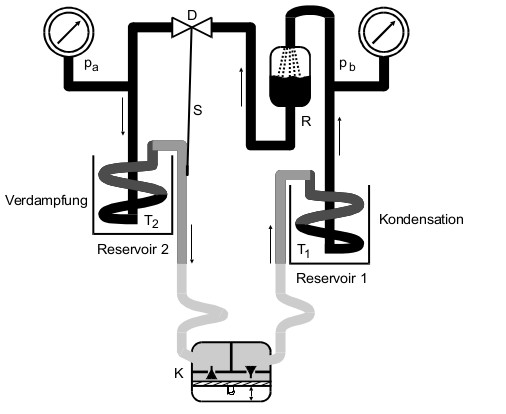
\includegraphics[width=0.75\linewidth]{./images/theo_Aufbau.jpg}
    \caption{prinzipieller Aufbau der Wärmepumpe ($p_a>p_b$;$T_1>T_2$) \cite{V206}} 
    \label{fig:1}
\end{figure}
Durch den Kompressor K entsteht ein Mediumkreislauf, während das Gas
durch das Drosselventil vom Reservoir 1 ins Reservoir 2 strömt.
Bei der Temperatur $T_1$ und dem Druck $p_b$ ist das Gas flüssig, während
es bei $T_2$ und $p_a$ gasförmig ist.\\
Eine Kenngröße zur Beschreibung der realen Wärmepumpe bildet die reale Güteziffer.
Um diese zu berechnen wird vorher die pro Zeiteinheit gewonnene Wärmemenge \cite{V206}
\begin{align}
    \frac{\Delta Q_1}{\Delta t}=(m_1 c_w+m_k c_k)\frac{\Delta T_1}{\Delta t} \label{eq:3}
\end{align}
berechnet. Dabei ist $m_1 c_w$ die Wärmekapazität des Wassers, $m_k c_k$ die
Wärmekapazität der Kupferschlange und des Eimers in der Abbildung und
$\sfrac{\Delta T_1}{Delta t} $ die zeitliche Änderung der Temperatur.
Damit wird Die Güteziffer $\nu$ berechnet:\cite{V206}
\begin{align}
    \nu_{real}= \frac{\Delta Q_1}{\Delta t N} \label{eq:4}
\end{align}
Dabei ist N die über dem Zeitintervall gemittelte Leistungsaufnahme des Kompressors.\\
Eine weitere wichtige Größe bildet der Massendurchsatz.\cite{V206}
\begin{align}
    L\frac{\Delta m}{\Delta t}&=\frac{\Delta Q_2}{\Delta t} \label{eq:5}
    \intertext{mit}
    \frac{\Delta Q_2}{\Delta t}&=(m_2 c_w+m_k c_k)\frac{\Delta T_2}{\Delta t} \label{eq:6}
\end{align}
Die Verdampfungswärme L wird dabei mit der Formel \cite{V203}
\begin{align}
    \ln(p)=- \frac{L}{R} \frac{1}{T}+const \label{eq:7}
\end{align}
unter der Annahme bestimmt, dass die Temperaturen weit unter der kritischen Temperatur liegen, 
das Volumen der Flüssigkeit gegenüber dem Volumen des Gases vernachlässigbar ist und das
Gasvolumen durch die ideale Gasgleichung \cite{V203}
\begin{align}
    V_D(p,T)=R \; \frac{T}{p} \label{eq:8}
\end{align}
beschrieben werden kann.\\
Die letze relevante Größe ist die mechanische Krompessorleistung $N_{mech} $, welche die
theoretische Größe der Leisung darstellt:\cite{V206}
\begin{align}
    N_{mech}=\frac{1}{\kappa-1}\left(p_b \sqrt[\kappa]{\frac{p_a}{p_b} -p_a}\right) \frac{1}{\rho} \frac{\Delta m}{\Delta t} \label{eq:9}
\end{align}
$\rho$ bezeichnet die Dichte des Mediums und $\kappa$ das Verhältnis der Molwärmen $C_p$ und $C_V$.

% Fehlerrechnung %%%%%%%%%%%%%%%%%%%%%%%%%%%%%%%%%%%%%%%%%%%%%%%%%%%%%%%%%%%%%%%%%%%%%%%%%%%%%%%%%%%%%%%%%%%%%%%%%%%%%%%%%%%%%%%%%%%%%%%%%%%%%%%%%%%%%%%%%%%%%%%%%%%%%%%%%%%%%%%%%%%%%%%%%%%%%%%%%%%%%%%%%%%%%%%%%%%%%%

\section{Fehlerrechnung}\justifying

Für die Berechnung von Messunsicherheiten werden in diesem Protokoll folgende Formeln
verwendet:
\begin{subequations} \label{eq:10}
\begin{align} 
\intertext{Zur Bestimmung eines Mittelwertes wird folgende Formel benutzt:
}
    \overline{x} &= \frac{1}{N}\sum_{i=1}^{N} x_i \label{eq:10a}
\intertext{Zur Bestimmung der Messunsicherheit bei Mittelwerten wird mit der Formel
}
    \Delta\overline{x} &= \frac{1}{\sqrt{N}} \sqrt{\frac{1}{1-N} \sum_{i=1}^{N} (x_i - \overline{x})^2} \label{eq:10b},
\intertext{gearbeitet und die Gaußsche Fehlerfortpflanzung wird mit
}
    \sigma _f &= \sqrt{\sum_{i=1}^{N} \left( \frac{\partial f}{\partial x_i} \right)^2 \cdot (\sigma_{x_i})^2} \label{eq:10c}
\intertext{berechnet. Um Ausgleichsgeraden und ihre Parameter zu bestimmen, werden folgende Formeln verwendet:
}
    y &= m \cdot x + b \label{eq:10d} \\ 
    m &= \frac{\overline{xy} - \overline{x} \cdot \overline{y}}{\overline{x^2} - {\overline{x}}^2} \label{eq:10e}\\
    b &= \frac{\overline{y} \cdot \overline{x^2} - \overline{xy} \cdot \overline{x}}{\overline{x^2} - {\overline{x}}^2} \label{eq:10f}
\end{align}
\end{subequations}
\newpage

% Versuchsaufbau + Versuchsdurchführung %%%%%%%%%%%%%%%%%%%%%%%%%%%%%%%%%%%%%%%%%%%%%%%%%%%%%%%%%%%%%%%%%%%%%%%%%%%%%%%%%%%%%%%%%%%%%%%%%%%%%%%%%%%%%%%%%%%%%%%%%%%%%%%%%%%%%%%%%%%%%%%%%%%%%%%%%%%%%%%%%%%%%%%%%%%%%%%%%%%%%%%%%%%%%%%%%%

\section{Versuchsaufbau und Versuchsdurchführung}\justifying

Benötigt werden: \textit{Zwei Manometer, zwei Thermometer, zwei Rührmotoren, zwei thermisch isolierte Wasserbehälter, ein Kompressor, 
ein Drosselventil, ein Reiniger, ein Wattmeter, eine Stoppuhr, ein Messkolben und $\SI{6}{\liter}$ Wasser.}

\flushleft{Das\;}\justifying Experiment wird wie in Abbildung \ref{fig:2} aufgebaut:

\begin{figure}
    \centering
    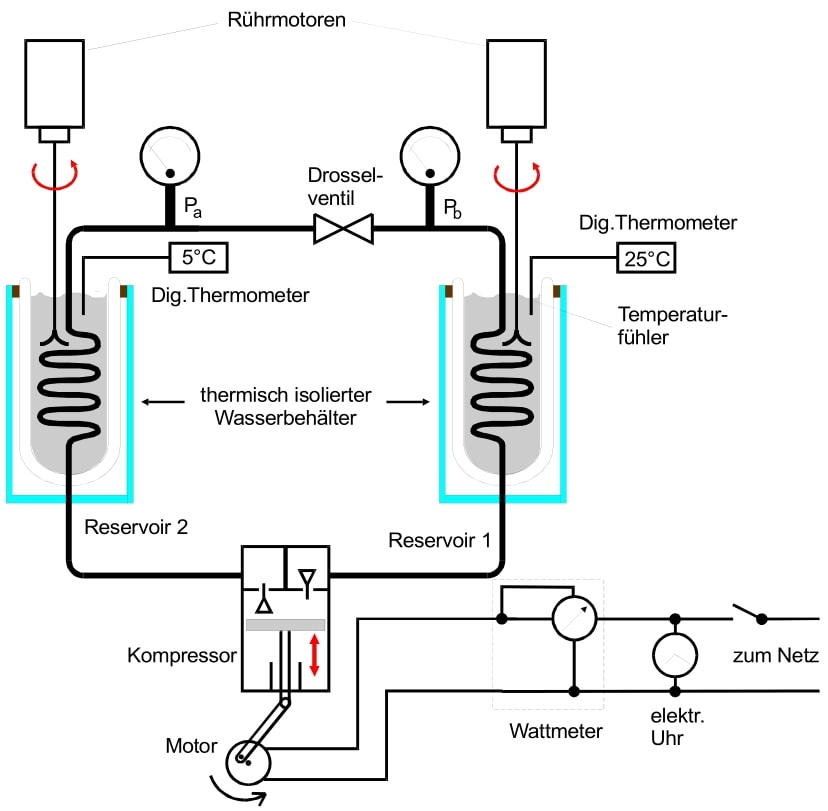
\includegraphics[width=0.75\linewidth]{./images/Aufbau.jpg}
    \caption{Versuchsaufbau der Wärmepumpe \cite{V206}}
    \label{fig:2}
\end{figure}

\flushleft{Außerdem\;}\justifying soll zwischen dem Manometer $P_b$ und dem Drosselventil ein Reiniger geschaltet werden. 

\flushleft{Zu\;}\justifying Beginn werden beide Wasserbehälter mit je drei Liter Wasser gefüllt. Diese werden um die zwei Spulen und
Rührmotoren platziert. Anschließend werden das Wattmeter und der Kompressor eingeschaltet. Mithilfe der Stoppuhr werden nun im Minutentakt
die Temperaturen der beiden Reservoire 1 und 2, die Drücke $P_a$ und $P_b$, und die erbrachte Leistung des Kompressors abgelesen. Es werden
solange Messwerte aufgenommen, bis die Temperatur in Reservoir 1 auf $\SI{50}{\celsius}$ gestiegen ist. 
Abschließend werden Wattmeter und Kompressor abgeschaltet und beide Reservoire geleert. 

% Auswertung %%%%%%%%%%%%%%%%%%%%%%%%%%%%%%%%%%%%%%%%%%%%%%%%%%%%%%%%%%%%%%%%%%%%%%%%%%%%%%%%%%%%%%%%%%%%%%%%%%%%%%%%%%%%%%%%%%%%%%%%%%%%%%%%%%%%%%%%%%%%%%%%%%%%%%%%%%%%%%%%%%%%%%%%%%%%%%%%%%%%%%%%%%%%%%%%%%

\section{Auswertung}
\begin{table}[H]
    \centering
    \input{table.tex}
    \caption{Messwerte der Wärmepumpe}
    \label{tab:1}
\end{table}
\newpage

\flushleft{Der\;}\justifying Temperaturverlauf der einzelnen Reservoire werden mithilfe der Messwerte in Tabelle \ref{tab:1} erstellt. Die für
die Graphen \ref{fig:3a} und \ref{fig:3b} relevanten Parameter $a$, $b$ und $c$ wurden mit dem Python Befehl np.ployfit() \cite{numpy}
berechnet und lauten wie folgt:
\begin{subequations}
\begin{align}
    a_{T1} &= \text{\input{parT1_a.tex}} \qquad &a_{T2} &= \text{\input{parT2_a.tex}} \label{eq:11a}\\
    b_{T1} &= \text{\input{parT1_b.tex}} \qquad &b_{T2} &= \text{\input{parT2_b.tex}} \label{eq:11b}\\
    c_{T1} &= \text{\input{parT1_c.tex}} \qquad &c_{T2} &= \text{\input{parT2_c.tex}} \label{eq:11c}
\end{align}
\end{subequations}

\begin{figure}[H]
    \begin{subfigure}{0.495\linewidth}
        \centering
        \includegraphics[width=\textwidth]{./build/plotT1.pdf}
        \caption{Lineare Regression der Temperatur $T_1$}
        \label{fig:3a}
    \end{subfigure}
    \begin{subfigure}{0.495\linewidth}
        \centering
        \includegraphics[width=\textwidth]{./build/plotT2.pdf}
        \caption{Lineare Regression der Temperatur $T_2$}
        \label{fig:3b}
    \end{subfigure}
    \caption{Lineare Regressionen der Temperaturen}
    \label{fig:3}
\end{figure}

\flushleft{Um\;}\justifying die zwei Differentialquotienten $\sfrac{dT_{1}}{dt}$ und $\sfrac{dT_{2}}{dt}$ zu berechnen, wird die Formel
\begin{align}
    \frac{dT(t)}{dt} = 2At + B \label{eq:12}
\end{align}
benötigt. Mit der gaußschen Fehlerfortpflanzung \eqref{eq:10c} folgt:
\begin{align}
    \sigma_{T_i} = \sqrt{4t^2 \cdot \sigma _{A_i}^2 + t^2 \cdot \sigma _{B_i}^2} \label{eq:13}\quad \text{mit}\; i = 1,2
\end{align}
Um mit der Fehlerfortpflanzung \eqref{eq:13} auf die Differentialquotienten $\sfrac{d_{T1}}{dt}$ und $\sfrac{d_{T2}}{dt}$ zu schließen werden die 
Temperaturen $\SI{26.6}{\celsius}$, $\SI{39.9}{\celsius}$, $\SI{46.7}{\celsius}$ und $\SI{49.6}{\celsius}$ für $T_1$ verwendet. Für $T_2$ 
werden die Temperaturen $\SI{17.4}{\celsius}$, $\SI{7.8}{\celsius}$, $\SI{1.4}{\celsius}$ und $\SI{-0.4}{\celsius}$ benutzt.
Die daraus folgenden Differentialquotienten lauten:
\begin{table}[H]
    \centering
    \input{build/tabledTdt.tex}
    \caption{zeitliche Veränderung der Temperatur} \label{tab:2}
\end{table}


\flushleft{Für\;}\justifying die Güteziffer wird die gemittelte Leistung $N$ des Kompressors benötigt. Diese wird mit den Messwerten aus Tabelle
\ref{tab:1} und der Mittelwertsformel \eqref{eq:10a} bestimmt. Die gemittelte Leistung lautet wie folgt:
\begin{align}
    N = \text{\input{P_mean.tex}} \label{eq:14}
\end{align}
Mithilfe der Formel \eqref{eq:4}, der gemittelten Leistung $N$ \eqref{eq:14} und der Fehlerfortpflanzung \eqref{eq:10c}
\begin{align}
    \sigma_{\nu_{real}} = \sqrt{\frac{1}{N^2} \cdot \sigma_{\frac{\Delta Q_i}{\Delta t}}^2 + \left( \frac{-\Delta Q_i}{\Delta t N^2} \right)^2 \cdot \sigma_{N}^2} \label{eq:15}
\end{align}
ergeben sich die in der Tabelle \ref{tab:3} aufgeführten Werte für $\nu_{real}$.

\begin{table}[H]
    \centering
    \input{table_calc.tex}
    \caption{Tabelle der Rechnungsergebnisse}
    \label{tab:3}
\end{table}

\flushleft{Für\;}\justifying den folgenden Graphen \ref{fig:4} der Verdampfungswärme von Dichlordifluormethan werden die Parameter $m$ und $b$ verwendet, wobei $m$ mit der
Formel \eqref{eq:10e} berechnet wird. Die Werte des Druckes und der Temperatur werden der Tabelle \ref{tab:1} entnommen. 
\begin{subequations}\label{eq:16}
\begin{align}
    m_L &= \text{\input{parL_m.tex}}\label{eq:16a}\\
    b_L &= \text{\input{parL_b.tex}}\label{eq:16b}
\end{align}
\end{subequations}

\begin{figure}[H]
    \centering
    \includegraphics[width=0.75\linewidth]{./build/plotL.pdf}
    \caption{Lineare Regression der Verdampfungswärme $L$}
    \label{fig:4}
\end{figure}

\flushleft{Die\;}\justifying Verdampfungswärme von Dichlordifluormethan lässt sich somit mit der Ausgleichsgeraden des Graphen \ref{fig:4}, 
der idealen Gasgleichung \eqref{eq:8} und der molaren Masse von Dichlordifluormethan $\SI{0.12091}{\kilo\gram\per\mole}$ \cite{Molmasse} bestimmen:
\begin{align}
    L = \text{\input{L.tex}}\label{eq:17}
\end{align}

\flushleft{Für\;}\justifying die mechanische Leistung $N_{mech}$ des Kompressors wird die Formel \eqref{eq:6} und die Dichlordifluormethan spezifischen Werte 
\cite{V206} $\rho_0 = \SI{5.51}{\gram\liter\tothe{-1}}, T = \SI{0}{\celsius}, p = \SI{1}{\bar}, \kappa = 1.14$ verwendet. Es werden die Drücke für die vorherig
verwendeten vier Zeiten ($\SI{4}{\second}, \SI{15}{\second}, \SI{25}{\second}, \SI{29}{\second}$) aus Tabelle \ref{tab:1} verwendet. Die daraus
folgenden mechanischen Leistungen betragen:
\begin{subequations}
\begin{align}
    N_{mech1} = \text{\input{N0.tex}} \label{eq:18a}\\
    N_{mech2} = \text{\input{N1.tex}} \label{eq:18b}\\
    N_{mech3} = \text{\input{N2.tex}} \label{eq:18c}\\
    N_{mech4} = \text{\input{N3.tex}} \label{eq:18d}
\end{align}
\end{subequations}



% Diskussion %%%%%%%%%%%%%%%%%%%%%%%%%%%%%%%%%%%%%%%%%%%%%%%%%%%%%%%%%%%%%%%%%%%%%%%%%%%%%%%%%%%%%%%%%%%%%%%%%%%%%%%%%%%%%%%%%%%%%%%%%%%%%%%%%%%%%%%%%%%%%%%%%%%%%%%%%%%%%%%%%%%%%%%%%%%%%%%%%%%%%%%%%%%%%%%%%%

\section{Diskussion}

% Literatur %%%%%%%%%%%%%%%%%%%%%%%%%%%%%%%%%%%%%%%%%%%%%%%%%%%%%%%%%%%%%%%%%%%%%%%%%%%%%%%%%%%%%%%%%%%%%%%%%%%%%%%%%%%%%%%%%%%%%%%%%%%%%%%%%%%%%%%%%%%%%%%%%%%%%%%%%%%%%%%%%%%%%%%%%%%%%%%%%%%%%%%%%%%%%%%%%%

\newpage
\printbibliography

\end{document}
